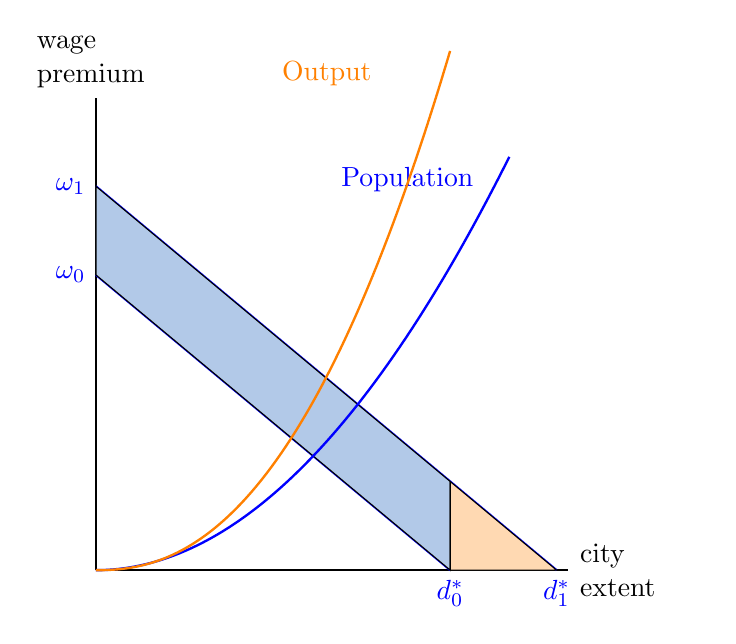
\begin{tikzpicture}[scale=.75]
\def\bndmax{8} 
\tikzset{func/.style={color=blue!80}}	
% EXTENT  BEFORE
\draw[thick](0,0)--(0,8)node[above, text width=1.5cm]{wage \newline premium}; % Y axis
\draw[thick](0,0)--(8,0)node[right=.5, text width=1.5cm]{city\newline extent};  % X axis
%\node at (3.5,-.7){Extent: Walkers};
\draw[thick, blue](0,5)node[left]{$\omega_0$}--(6,0)node[below]{$d^*_0$};
\draw[ thick, blue](0,{5*1.3})node[left]{$\omega_1$}--({6*1.3},0)node[below]{$d^*_1$};
\draw[fill=green!30!blue!30](0,5)--(0,{5*1.3})--(6,5*0.3)--(6,0)--cycle;
\draw[fill=orange!30]({6*1.3},0)--(6,5*0.3)--(6,0)--cycle;
\draw[func, domain=0:7, line width=.3mm,blue, text width=2cm] plot [samples=200] (\x,{\x^2/7})node[below left]{Population};
\draw[func,  domain=0:6, line width=.3mm, orange, text width=2cm] plot [samples=200] (\x,{\x^2.3/7})node[below left]{Output};
%\node[circle,draw=black, fill=white, inner sep=3pt,minimum size=10pt] (b) at (1,2.5) {1};
\end{tikzpicture}